\begin{atiTask}[
  title = Oberflächenintegral
  %call = Zusatzaufgabe,
]

Gegeben sei das Vektorfeld 
\[
\vec{\Phi}=xy\vec{i}+xz\vec{j}+yz\vec{k}
\]
sowie als Fläche $F$ das Dreieck mit Eckpunkten $(1,0,0)$, $(0,1,0)$ und $(0,0,2)$. Berechnen Sie 
\[
\iint_F \curl \vec{\Phi}\cdot \D\vec{f}.
\]

\atiNote{Erinnerung: Flächen dürfen deformiert werden.}

\end{atiTask}

\begin{atiSolution}
	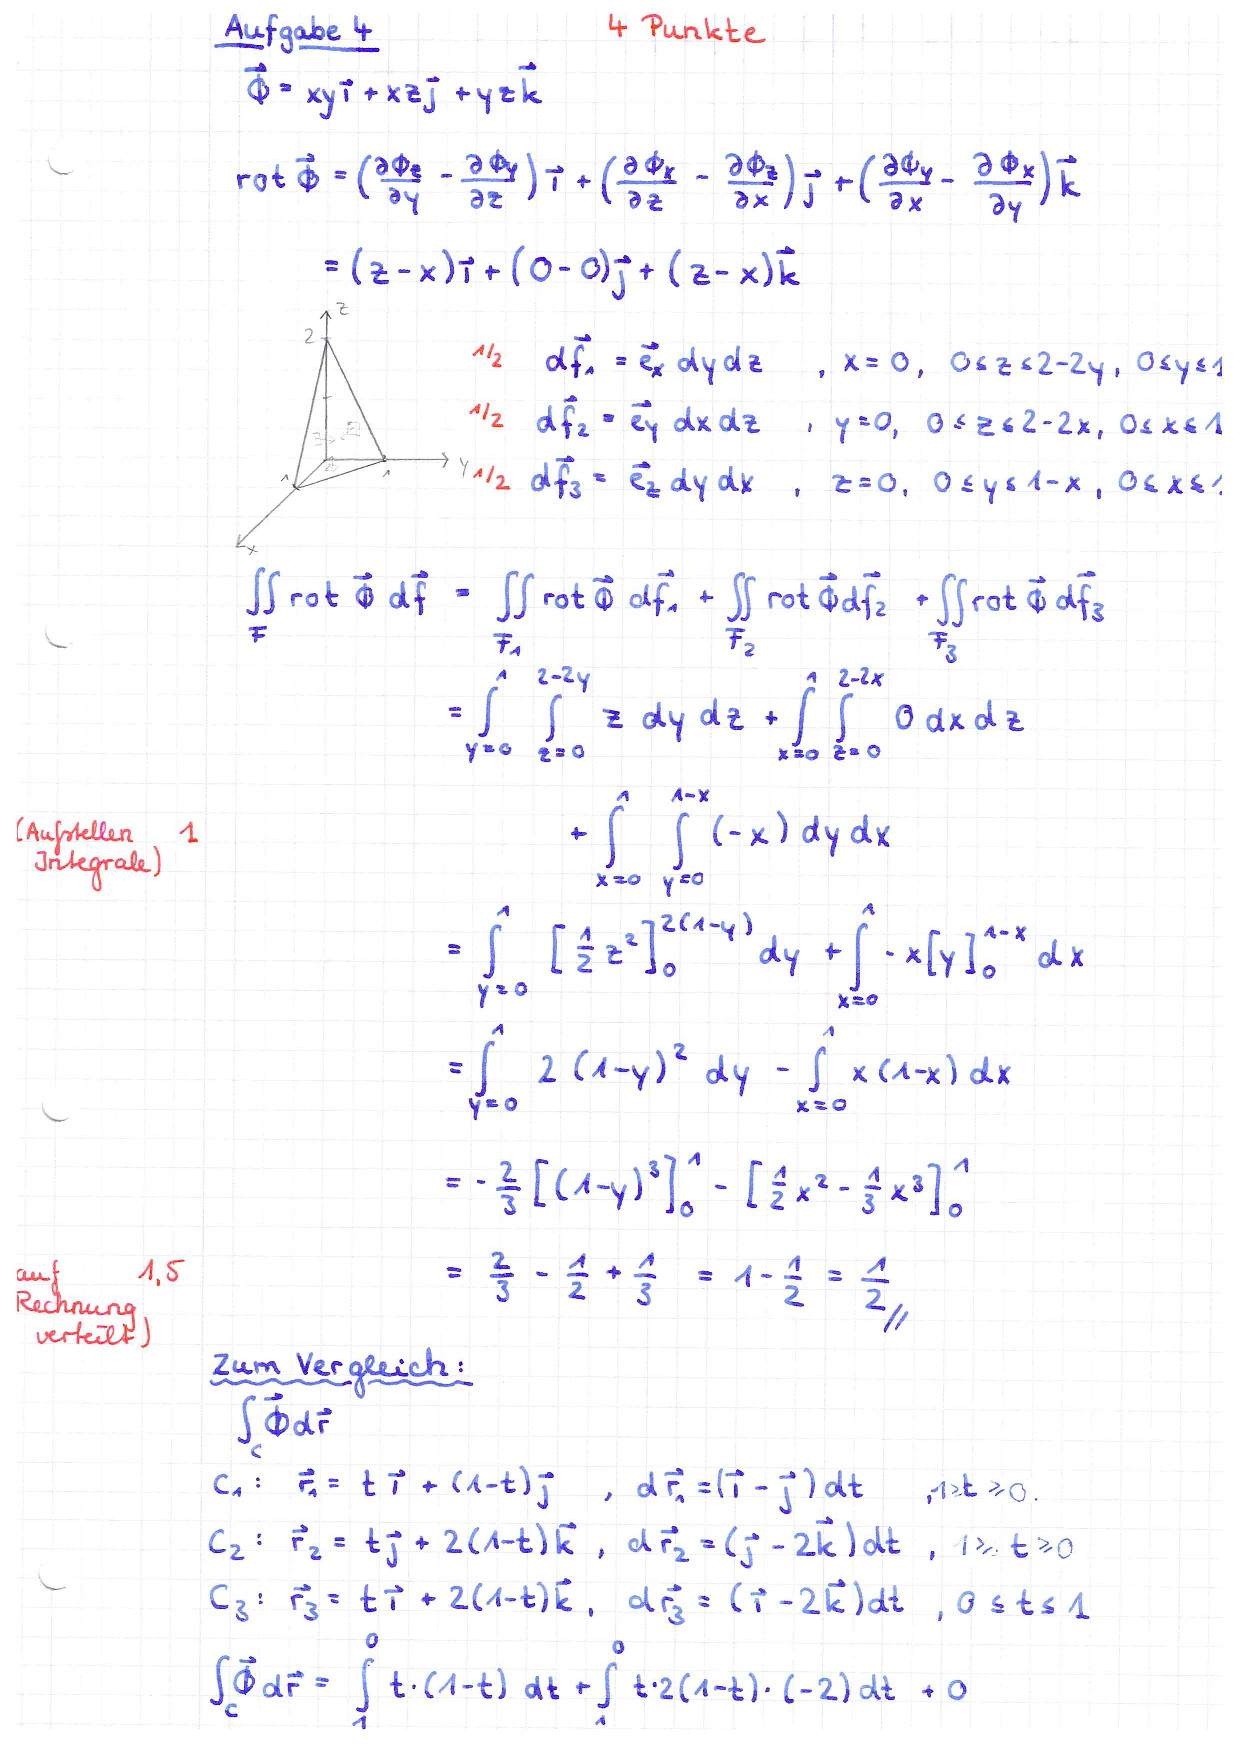
\includepdf{solution-stokes_v.pdf}
\end{atiSolution}